%===============================================================================
% LaTeX sjabloon voor de bachelorproef toegepaste informatica aan HOGENT
% Meer info op https://github.com/HoGentTIN/latex-hogent-report
%===============================================================================

\documentclass[dutch,dit,thesis]{hogentreport}

% TODO:
% - If necessary, replace the option `dit`' with your own department!
%   Valid entries are dbo, dbt, dgz, dit, dlo, dog, dsa, soa
% - If you write your thesis in English (remark: only possible after getting
%   explicit approval!), remove the option "dutch," or replace with "english".

\usepackage{lipsum} % For blind text, can be removed after adding actual content
\usepackage{listings}
\usepackage{xcolor}

% Define the custom colors
\definecolor{codegreen}{rgb}{0,0.6,0}
\definecolor{codegray}{rgb}{0.5,0.5,0.5}
\definecolor{codepurple}{rgb}{0.58,0,0.82}
\definecolor{backcolour}{rgb}{0.95,0.95,0.92}

% Define a listing style using these colors
\lstdefinestyle{coloredpython}{
    backgroundcolor=\color{backcolour},
    commentstyle=\color{codegreen},
    keywordstyle=\color{magenta}, % Keywords like def, import, for, if, etc.
    numberstyle=\tiny\color{codegray},
    stringstyle=\color{codepurple}, % Strings like "hello"
    basicstyle=\ttfamily\footnotesize, % Font style and size
    breaklines=true, % Wrap long lines
    captionpos=b, % Caption position (bottom)
    numbers=left, % Line numbers on the left
    numbersep=5pt, % Space between line numbers and code
    showspaces=false,
    showstringspaces=false,
    showtabs=false,
    tabsize=2, % Tab size
    language=Python % Set default language to Python
}
\lstset{style=coloredpython}

%% Pictures to include in the text can be put in the graphics/ folder
\graphicspath{{../graphics/}}
%% For source code highlighting, requires pygments to be installed
%% Compile with the -shell-escape flag!
%% \usepackage[chapter]{minted}
%% If you compile with the make_thesis.{bat,sh} script, use the following
%% import instead:
\usepackage[chapter,outputdir=../output]{minted}
\usemintedstyle{solarized-light}

%% Formatting for minted environments.
\setminted{%
    autogobble,
    frame=lines,
    breaklines,
    linenos,
    tabsize=4
}

%% Ensure the list of listings is in the table of contents
\renewcommand\listoflistingscaption{%
    \IfLanguageName{dutch}{Lijst van codefragmenten}{List of listings}
}
\renewcommand\listingscaption{%
    \IfLanguageName{dutch}{Codefragment}{Listing}
}
\renewcommand*\listoflistings{%
    \cleardoublepage\phantomsection\addcontentsline{toc}{chapter}{\listoflistingscaption}%
    \listof{listing}{\listoflistingscaption}%
}

% Other packages not already included can be imported here

%%---------- Document metadata -------------------------------------------------
% TODO: Replace this with your own information
\author{Tom Deganck}
\supervisor{Dhr. S. Lievens}
\cosupervisor{Mevr. K. Van Mele}
\title[]%
    {\sloppy{Real-time vertaling van Vlaamse Gebarentaal naar tekst op een mobiel apparaat}}%
\academicyear{\advance\year by -1 \the\year--\advance\year by 1 \the\year}
\examperiod{1}
\degreesought{\IfLanguageName{dutch}{Professionele bachelor in de toegepaste informatica}{Bachelor of applied computer science}}
\partialthesis{false} %% To display 'in partial fulfilment'
%\institution{Internshipcompany BVBA.}

%% Add global exceptions to the hyphenation here
\hyphenation{back-slash}

%% The bibliography (style and settings are  found in hogentthesis.cls)
\addbibresource{bachproef.bib}            %% Bibliography file
\addbibresource{../voorstel/voorstel.bib} %% Bibliography research proposal
\defbibheading{bibempty}{}

%% Prevent empty pages for right-handed chapter starts in twoside mode
\renewcommand{\cleardoublepage}{\clearpage}

\renewcommand{\arraystretch}{1.2}

%% Content starts here.
\begin{document}

%---------- Front matter -------------------------------------------------------

\frontmatter

\hypersetup{pageanchor=false} %% Disable page numbering references
%% Render a Dutch outer title page if the main language is English
\IfLanguageName{english}{%
    %% If necessary, information can be changed here
    \degreesought{Professionele Bachelor toegepaste informatica}%
    \begin{otherlanguage}{dutch}%
       \maketitle%
    \end{otherlanguage}%
}{}

%% Generates title page content
\maketitle
\hypersetup{pageanchor=true}

%%=============================================================================
%% Voorwoord
%%=============================================================================

\chapter*{\IfLanguageName{dutch}{Woord vooraf}{Preface}}%
\label{ch:voorwoord}

%% TODO:
%% Het voorwoord is het enige deel van de bachelorproef waar je vanuit je
%% eigen standpunt (``ik-vorm'') mag schrijven. Je kan hier bv. motiveren
%% waarom jij het onderwerp wil bespreken.
%% Vergeet ook niet te bedanken wie je geholpen/gesteund/... heeft

\lipsum[1-2]
%%=============================================================================
%% Samenvatting
%%=============================================================================

% TODO: De "abstract" of samenvatting is een kernachtige (~ 1 blz. voor een
% thesis) synthese van het document.
%
% Een goede abstract biedt een kernachtig antwoord op volgende vragen:
%
% 1. Waarover gaat de bachelorproef?
% 2. Waarom heb je er over geschreven?
% 3. Hoe heb je het onderzoek uitgevoerd?
% 4. Wat waren de resultaten? Wat blijkt uit je onderzoek?
% 5. Wat betekenen je resultaten? Wat is de relevantie voor het werkveld?
%
% Daarom bestaat een abstract uit volgende componenten:
%
% - inleiding + kaderen thema
% - probleemstelling
% - (centrale) onderzoeksvraag
% - onderzoeksdoelstelling
% - methodologie
% - resultaten (beperk tot de belangrijkste, relevant voor de onderzoeksvraag)
% - conclusies, aanbevelingen, beperkingen
%
% LET OP! Een samenvatting is GEEN voorwoord!

%%---------- Nederlandse samenvatting -----------------------------------------
%
% TODO: Als je je bachelorproef in het Engels schrijft, moet je eerst een
% Nederlandse samenvatting invoegen. Haal daarvoor onderstaande code uit
% commentaar.
% Wie zijn bachelorproef in het Nederlands schrijft, kan dit negeren, de inhoud
% wordt niet in het document ingevoegd.

\IfLanguageName{english}{%
\selectlanguage{dutch}
\chapter*{Samenvatting}
\lipsum[1-4]
\selectlanguage{english}
}{}

%%---------- Samenvatting -----------------------------------------------------
% De samenvatting in de hoofdtaal van het document

\chapter*{\IfLanguageName{dutch}{Samenvatting}{Abstract}}

\lipsum[1-4]


%---------- Inhoud, lijst figuren, ... -----------------------------------------

\tableofcontents

% In a list of figures, the complete caption will be included. To prevent this,
% ALWAYS add a short description in the caption!
%
%  \caption[short description]{elaborate description}
%
% If you do, only the short description will be used in the list of figures

\listoffigures

% If you included tables and/or source code listings, uncomment the appropriate
% lines.
\listoftables

\listoflistings

% Als je een lijst van afkortingen of termen wil toevoegen, dan hoort die
% hier thuis. Gebruik bijvoorbeeld de ``glossaries'' package.
% https://www.overleaf.com/learn/latex/Glossaries

%---------- Kern ---------------------------------------------------------------

\mainmatter{}

% De eerste hoofdstukken van een bachelorproef zijn meestal een inleiding op
% het onderwerp, literatuurstudie en verantwoording methodologie.
% Aarzel niet om een meer beschrijvende titel aan deze hoofdstukken te geven of
% om bijvoorbeeld de inleiding en/of stand van zaken over meerdere hoofdstukken
% te verspreiden!

%%=============================================================================
%% Inleiding
%%=============================================================================

\chapter{\IfLanguageName{dutch}{Inleiding}{Introduction}}%
\label{ch:inleiding}

De inleiding moet de lezer net genoeg informatie verschaffen om het onderwerp te begrijpen en in te zien waarom de onderzoeksvraag de moeite waard is om te onderzoeken. In de inleiding ga je literatuurverwijzingen beperken, zodat de tekst vlot leesbaar blijft. Je kan de inleiding verder onderverdelen in secties als dit de tekst verduidelijkt. Zaken die aan bod kunnen komen in de inleiding~\autocite{Pollefliet2011}:

\begin{itemize}
  \item context, achtergrond
  \item afbakenen van het onderwerp
  \item verantwoording van het onderwerp, methodologie
  \item probleemstelling
  \item onderzoeksdoelstelling
  \item onderzoeksvraag
  \item \ldots
\end{itemize}

\section{\IfLanguageName{dutch}{Probleemstelling}{Problem Statement}}%
\label{sec:probleemstelling}

Uit je probleemstelling moet duidelijk zijn dat je onderzoek een meerwaarde heeft voor een concrete doelgroep. De doelgroep moet goed gedefinieerd en afgelijnd zijn. Doelgroepen als ``bedrijven,'' ``KMO's'', systeembeheerders, enz.~zijn nog te vaag. Als je een lijstje kan maken van de personen/organisaties die een meerwaarde zullen vinden in deze bachelorproef (dit is eigenlijk je steekproefkader), dan is dat een indicatie dat de doelgroep goed gedefinieerd is. Dit kan een enkel bedrijf zijn of zelfs één persoon (je co-promotor/opdrachtgever).

\section{\IfLanguageName{dutch}{Onderzoeksvraag}{Research question}}%
\label{sec:onderzoeksvraag}

Wees zo concreet mogelijk bij het formuleren van je onderzoeksvraag. Een onderzoeksvraag is trouwens iets waar nog niemand op dit moment een antwoord heeft (voor zover je kan nagaan). Het opzoeken van bestaande informatie (bv. ``welke tools bestaan er voor deze toepassing?'') is dus geen onderzoeksvraag. Je kan de onderzoeksvraag verder specifiëren in deelvragen. Bv.~als je onderzoek gaat over performantiemetingen, dan 

\section{\IfLanguageName{dutch}{Onderzoeksdoelstelling}{Research objective}}%
\label{sec:onderzoeksdoelstelling}

Wat is het beoogde resultaat van je bachelorproef? Wat zijn de criteria voor succes? Beschrijf die zo concreet mogelijk. Gaat het bv.\ om een proof-of-concept, een prototype, een verslag met aanbevelingen, een vergelijkende studie, enz.

\section{\IfLanguageName{dutch}{Opzet van deze bachelorproef}{Structure of this bachelor thesis}}%
\label{sec:opzet-bachelorproef}

% Het is gebruikelijk aan het einde van de inleiding een overzicht te
% geven van de opbouw van de rest van de tekst. Deze sectie bevat al een aanzet
% die je kan aanvullen/aanpassen in functie van je eigen tekst.

De rest van deze bachelorproef is als volgt opgebouwd:

In Hoofdstuk~\ref{ch:stand-van-zaken} wordt een overzicht gegeven van de stand van zaken binnen het onderzoeksdomein, op basis van een literatuurstudie.

In Hoofdstuk~\ref{ch:methodologie} wordt de methodologie toegelicht en worden de gebruikte onderzoekstechnieken besproken om een antwoord te kunnen formuleren op de onderzoeksvragen.

% TODO: Vul hier aan voor je eigen hoofstukken, één of twee zinnen per hoofdstuk

In Hoofdstuk~\ref{ch:conclusie}, tenslotte, wordt de conclusie gegeven en een antwoord geformuleerd op de onderzoeksvragen. Daarbij wordt ook een aanzet gegeven voor toekomstig onderzoek binnen dit domein.
\chapter{\IfLanguageName{dutch}{Stand van zaken}{State of the art}}%
\label{ch:stand-van-zaken}

% Tip: Begin elk hoofdstuk met een paragraaf inleiding die beschrijft hoe
% dit hoofdstuk past binnen het geheel van de bachelorproef. Geef in het
% bijzonder aan wat de link is met het vorige en volgende hoofdstuk.

% Pas na deze inleidende paragraaf komt de eerste sectiehoofding.

Dit hoofdstuk bevat je literatuurstudie. De inhoud gaat verder op de inleiding, maar zal het onderwerp van de bachelorproef *diepgaand* uitspitten. De bedoeling is dat de lezer na lezing van dit hoofdstuk helemaal op de hoogte is van de huidige stand van zaken (state-of-the-art) in het onderzoeksdomein. Iemand die niet vertrouwd is met het onderwerp, weet nu voldoende om de rest van het verhaal te kunnen volgen, zonder dat die er nog andere informatie moet over opzoeken \autocite{Pollefliet2011}.

Je verwijst bij elke bewering die je doet, vakterm die je introduceert, enz.\ naar je bronnen. In \LaTeX{} kan dat met het commando \texttt{$\backslash${textcite\{\}}} of \texttt{$\backslash${autocite\{\}}}. Als argument van het commando geef je de ``sleutel'' van een ``record'' in een bibliografische databank in het Bib\LaTeX{}-formaat (een tekstbestand). Als je expliciet naar de auteur verwijst in de zin (narratieve referentie), gebruik je \texttt{$\backslash${}textcite\{\}}. Soms is de auteursnaam niet expliciet een onderdeel van de zin, dan gebruik je \texttt{$\backslash${}autocite\{\}} (referentie tussen haakjes). Dit gebruik je bv.~bij een citaat, of om in het bijschrift van een overgenomen afbeelding, broncode, tabel, enz. te verwijzen naar de bron. In de volgende paragraaf een voorbeeld van elk.

\textcite{Knuth1998} schreef een van de standaardwerken over sorteer- en zoekalgoritmen. Experten zijn het erover eens dat cloud computing een interessante opportuniteit vormen, zowel voor gebruikers als voor dienstverleners op vlak van informatietechnologie~\autocite{Creeger2009}.

Let er ook op: het \texttt{cite}-commando voor de punt, dus binnen de zin. Je verwijst meteen naar een bron in de eerste zin die erop gebaseerd is, dus niet pas op het einde van een paragraaf.

\begin{figure}
  \centering
  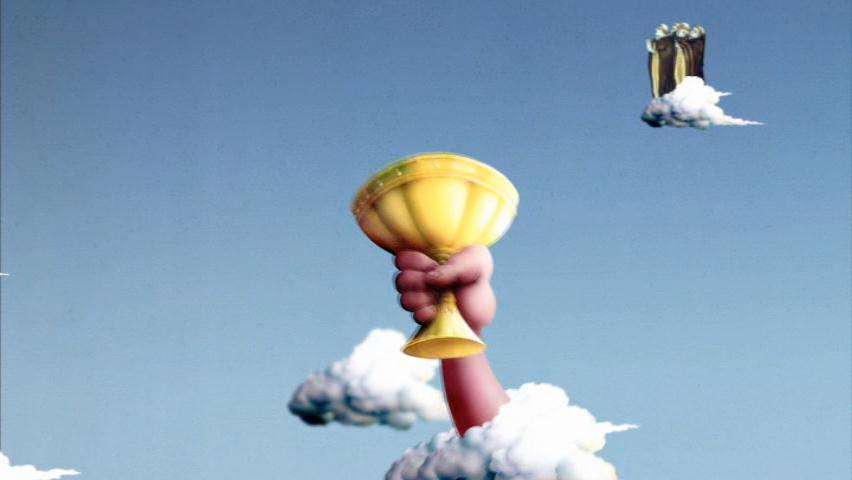
\includegraphics[width=0.8\textwidth]{grail.jpg}
  \caption[Voorbeeld figuur.]{\label{fig:grail}Voorbeeld van invoegen van een figuur. Zorg altijd voor een uitgebreid bijschrift dat de figuur volledig beschrijft zonder in de tekst te moeten gaan zoeken. Vergeet ook je bronvermelding niet!}
\end{figure}

\begin{listing}
  \begin{minted}{python}
    import pandas as pd
    import seaborn as sns

    penguins = sns.load_dataset('penguins')
    sns.relplot(data=penguins, x="flipper_length_mm", y="bill_length_mm", hue="species")
  \end{minted}
  \caption[Voorbeeld codefragment]{Voorbeeld van het invoegen van een codefragment.}
\end{listing}

\lipsum[7-20]

\begin{table}
  \centering
  \begin{tabular}{lcr}
    \toprule
    \textbf{Kolom 1} & \textbf{Kolom 2} & \textbf{Kolom 3} \\
    $\alpha$         & $\beta$          & $\gamma$         \\
    \midrule
    A                & 10.230           & a                \\
    B                & 45.678           & b                \\
    C                & 99.987           & c                \\
    \bottomrule
  \end{tabular}
  \caption[Voorbeeld tabel]{\label{tab:example}Voorbeeld van een tabel.}
\end{table}


%%=============================================================================
%% Methodologie
%%=============================================================================

\chapter{\IfLanguageName{dutch}{Methodologie}{Methodology}}%
\label{ch:methodologie}

%% TODO: In dit hoofdstuk geef je een korte toelichting over hoe je te werk bent
%% gegaan. Verdeel je onderzoek in grote fasen, en licht in elke fase toe wat
%% de doelstelling was, welke deliverables daaruit gekomen zijn, en welke
%% onderzoeksmethoden je daarbij toegepast hebt. Verantwoord waarom je
%% op deze manier te werk gegaan bent.
%% 
%% Voorbeelden van zulke fasen zijn: literatuurstudie, opstellen van een
%% requirements-analyse, opstellen long-list (bij vergelijkende studie),
%% selectie van geschikte tools (bij vergelijkende studie, "short-list"),
%% opzetten testopstelling/PoC, uitvoeren testen en verzamelen
%% van resultaten, analyse van resultaten, ...
%%
%% !!!!! LET OP !!!!! 
%% Het is uitdrukkelijk NIET de bedoeling dat je het grootste deel van de corpus 
%% van je bachelorproef in dit hoofdstuk verwerkt! Dit hoofdstuk is eerder een 
%% kort overzicht van je plan van aanpak.
%% Maak voor elke fase (behalve het literatuuronderzoek) een NIEUW HOOFDSTUK aan
%% en geef het een gepaste titel.

\section{Fase 1: App-ontwikkeling en modelselectie}
In de eerste fase van het onderzoek ligt de focus op het ontwikkelen van een applicatie die de camera kan gebruiken voor het verwerken van gebaren. De applicatie zal fungeren als de interface tussen de gebruiker en het model, en zorgt ervoor dat de camera-beeldgegevens van de gebruiker kunnen worden vastgelegd en verwerkt.

Daarnaast wordt er gezocht naar een geschikt deep learning-model dat in staat is om gebarentaal te herkennen en om te zetten in tekst. Dit model zal worden gekozen op basis van de literatuurstudie en de beschikbaarheid van bestaande, pre-getrainde modellen. Er zal een focus liggen op de effectiviteit van het model in termen van nauwkeurigheid en snelheid, zodat het geschikt is voor gebruik in real-time toepassingen.

Deze fase zal een periode van 2 weken innemen, waarin het ontwikkelen van de app en het selecteren van een geschikt model centraal staan, evenals het uitvoeren van initiële tests met het model \ref{fig:flowchart_tijd}.

\section{Fase 2: Modeloptimalisatie}
In de tweede fase van het onderzoek zal het gekozen model geoptimaliseerd worden om efficiënter te werken. 
Dit gebeurt door parameters en architectuurcomponenten, zoals het aantal en type lagen, te analyseren en indien nodig aan te passen. 
De optimalisatie is gericht op het verbeteren van de snelheid en efficiëntie, zodat het model beter geschikt is voor gebruik op mobiele apparaten.

Daarnaast worden technieken zoals pruning en quantization onderzocht om het model geschikt te maken voor de beperkte rekenkracht van mobiele apparaten. 
Deze technieken helpen bij het verkleinen van het model en verbeteren de prestaties zonder concessies te doen aan de nauwkeurigheid.

Voordat het model wordt geïntegreerd in de applicatie, zal het eerst worden getest in een Python-notebook. 
Dit stelt ons in staat om de basisfunctionaliteit en nauwkeurigheid van het model te evalueren zonder de complexiteit van de mobiele implementatie. 
Door eerst tests in de notebook uit te voeren, kunnen we een solide basis leggen en ervoor zorgen dat de performance voldoet aan de vereisten.

Op basis van de testresultaten kunnen eventuele aanpassingen worden doorgevoerd voordat het model verder geoptimaliseerd wordt en later in de app wordt geïntegreerd.

Deze fase zal 6 weken duren, waarin zowel de modeloptimalisatie als de testen plaatsvinden, inclusief de aanpassingen op basis van de testresultaten en performanceverbeteringen \ref{fig:flowchart_tijd}.

\section{Fase 3: Model implementeren in de app}
In deze fase wordt het geoptimaliseerde model geïntegreerd in de applicatie. 
Dit is een cruciale stap, aangezien het model nu operationeel moet worden in een echte applicatieomgeving op een mobiel apparaat.

De eerste stap is het exporteren van het model naar een geschikt formaat, zoals TensorFlow Lite of ONNX, zodat het gemakkelijk in de app kan worden geladen. 
Vervolgens wordt het model geïmplementeerd in de applicatiecode en getest op de app-omgeving.

De applicatie wordt geconfigureerd zodat de camera-feed van de gebruiker wordt gekoppeld aan het model voor real-time gebarentaalherkenning. 

Deze fase is essentieel voor het testen van de interactie tussen de applicatie, de camera, en het model, en zal helpen bij het identificeren van eventuele problemen met de integratie.

Deze fase zal vier weken duren, waarin de integratie van het model in de app en het testen van de interacties plaatsvindt \ref{fig:flowchart_tijd}.

\section{Fase 4: Evaluatie \& Validatie}
In de laatste fase van het onderzoek wordt het model geëvalueerd en gevalideerd. 
Dit gebeurt door middel van tests op een aparte dataset om de nauwkeurigheid en real-time prestaties te meten. 
De focus ligt hierbij op het testen van het model op ongeziene data om de generaliseerbaarheid en robuustheid van het model te waarborgen.

Daarnaast zal het model worden getest in real-time omstandigheden om te beoordelen hoe goed het functioneert bij het verwerken van live camera-invoer. 
Eventuele tekortkomingen in het model worden geanalyseerd en indien nodig verbeterd.

Deze fase zal 2 weken duren, waarin de tests op een aparte dataset en de real-time validatie plaatsvinden, gevolgd door het analyseren van de testresultaten en het doorvoeren van verbeteringen indien nodig \ref{fig:flowchart_tijd}.

\begin{figure}[h!]
  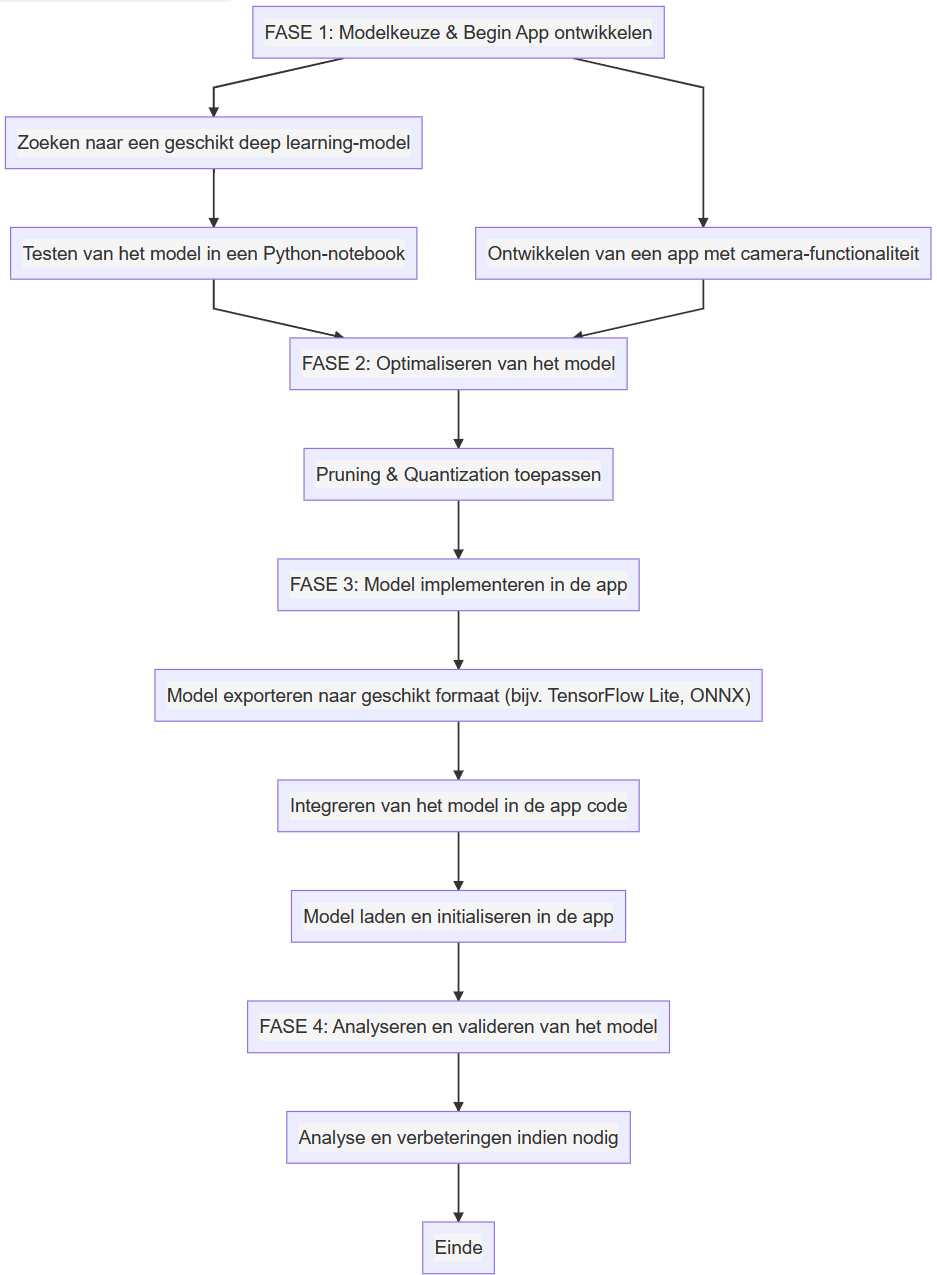
\includegraphics[width=1\textwidth]{../graphics/flowchart.png}
  \caption{Tijdlijn van het onderzoek}
  \label{fig:flowchart_tijd}
\end{figure}


% Voeg hier je eigen hoofdstukken toe die de ``corpus'' van je bachelorproef
% vormen. De structuur en titels hangen af van je eigen onderzoek. Je kan bv.
% elke fase in je onderzoek in een apart hoofdstuk bespreken.

%\input{...}
%\input{...}
%...
\chapter{\IfLanguageName{dutch}{Training van het model}{Training the model}}
\label{ch:trainingvhmodel}
Voordat het model gebruikt kan worden moet het eerst getraind worden.
Dit gebeurt door het model te voeden met een dataset van video's en hun bijhorende uitkomsten.
Bij dit model is de dataset al reeds gepreprocessed en in een formaat dat het model kan gebruiken.
Dit is echter nadelig voor ons omdat we niet weten hoe de data is gepreprocessed.
Waardoor het bij de inferentie moeilijker is om de data te pre-processen.

\section{Dataset}
\label{sec:dataset}

De dataset die gebruikt wordt is de \textit{RWTH-PHOENIX-Weather 2014 T} \footnote{\url{https://www-i6.informatik.rwth-aachen.de/~koller/RWTH-PHOENIX-2014-T/}} dataset.
Dit is een veelgebruikte dataset voor het trainen van gebarentaalmodellen.
De dataset bevat video's van het Duits gebarentaal en hun bijhorende transcripties.
De video's zijn extracties van het weerbericht van de Duitse publieke omroep PHOENIX.
\\
\\
De reden voor een Duitse dataset is omdat in het Vlaams gebarentaal geen goed genoege dataset bestaat.
Deze dataset wordt ook meestal gebruikt als benchmark voor gebarentaalmodellen.
Dit is samen met de RWTH-PHOENIX-Weather 2014\footnote{\url{https://www-i6.informatik.rwth-aachen.de/~koller/RWTH-PHOENIX/}} dataset en de CSL-Daily\footnote{\url{https://ustc-slr.github.io/datasets/2021_csl_daily/}} dataset de meest voorkomende dataset om gebarentaalmodellen te testen.
\\
\\
De github van het model geeft echter een link naar een kleinere subset van de dataset.
Het SignFormer model is gebouwd om met deze subset te werken en niet met de volledige dataset.
De precieze manier waarop de dataset is gepreprocessed is te vinden in een totaal andere paper namelijk:\textcite{SLTS}.
Echter staat hier ook niet exact uitgelegd hoe de data is gepreprocessed.
Er kan wel een schatting gemaakt worden van hoe de data is gepreprocessed.
Deze schatting wordt dan ook effectief gebruikt in de inferentie.


\section{Training}
\label{sec:training}
Voor het trainen van het model is er een aantal hyperparameters ingesteld.
De hyperparameters zijn:
\begin{itemize}
  \item Feature size: 1024
  \item Learning rate: 0.0004
  \item Epochs: 1000
  \item Max Sentence Length: 400
  \item Eval metric: bleu
  \item Batch size: 32
  \item Early stopping: eval metric
  \item translation beam sizes: 1, ..., 10
  \item translation beam alpha's: -1, ..., 5
\end{itemize}

De ingestelde hyperparameters definiëren belangrijke aspecten van het trainingsproces en de architectuur van het model voor gebarentaalherkenning. 
De 'Feature size' van 1024 bepaalt de dimensionaliteit van de feature vectoren die worden geëxtraheerd uit de input data (zoals videoframes of sequenties die gebaren vertegenwoordigen). 
Deze vector van 1024 elementen representeert de kenmerken (visuele aspecten, beweging) van de input op een bepaald moment of segment, die relevant zijn voor het herkennen van het gebaar. 
Een hogere waarde staat toe complexere visuele of temporele kenmerken vast te leggen.
De keuze voor 1024 hangt dus af van het formaat van de voorverwerkte dataset.
\\
De 'Learning rate' van 0.0004 is een cruciale parameter voor de optimalisatie: het bepaalt de stapgrootte waarmee de gewichten van het model aangepast worden tijdens het leren. 
Een kleine waarde zoals 0.0004 zorgt vaak voor stabiele convergentie.
\\
Het aantal 'Epochs' is ingesteld op 1000, wat aangeeft dat het model potentieel 1000 keer de gehele trainingsdataset doorloopt. 
Echter, door gebruik te maken van 'Early stopping', zal de training waarschijnlijk eerder stoppen om overfitting te voorkomen.
\\
'Early stopping' is geconfigureerd om te reageren op de 'Eval metric', wat betekent dat de training stopt zodra de prestatie op de validatieset, gemeten met de 'bleu' score, niet meer verbetert. 
Het gebruik van 'bleu' (Bilingual Evaluation Understudy) als evaluatiemetriek suggereert dat het model mogelijk getraind wordt voor gebarentaal vertaling naar tekst, aangezien BLEU een veelgebruikte metriek is voor het evalueren van de kwaliteit van gegenereerde tekst.
\\
De 'Max Sentence Length' van 400 specificeert de maximale lengte van de inputsequenties in termen van tijdstappen of frames. 
Dit is dus de maximale duur van een gebaar of een reeks gebaren die het model in één keer kan verwerken. 
Langere sequenties worden typisch afgekapt en kortere worden aangevuld (padding).
\\
Tot slot definieert de 'Batch size' van 32 het aantal trainingsvoorbeelden (oftewel sequenties van gebarendata) dat gezamenlijk door het model wordt verwerkt in één iteratie voordat de modelgewichten worden bijgewerkt. 
Samen bepalen deze parameters hoe het model leert en presteert op de gebarentaalherkenningstaak.

\subsubsection{Andere training parameters}
Naast de hyperparameters zijn er ook andere parameters ingesteld voor het trainen van het model.
Dit zijn vooral parameters voor het model zelf.
De parameters zijn:
\begin{itemize}
  \item encoder
  \begin{itemize}
    \item layers: 1
    \item type: transformer
    \item attention heads: 8
    \item embeddings size: 256
    \item activation: softsign
  \end{itemize}
  \item decoder
  \begin{itemize}
    \item layers: 1
    \item type: transformer
    \item attention heads: 8
    \item embeddings size: 256
    \item activation: softsign
  \end{itemize}
\end{itemize}

De parameters zijn ingesteld om de architectuur van het model te definiëren.
De encoder en decoder zijn beide transformer-gebaseerd, wat betekent dat ze gebruik maken van self-attention mechanismen om de relaties tussen verschillende delen van de inputsequentie te begrijpen.


\section{Resultaten}
\label{sec:results}
Na het trainen van het model zijn er verschillende evaluaties uitgevoerd om de prestaties van het model te meten.
Deze evaluaties zijn gemaakt op een computer met een NVIDIA GeForce RTX 3050 Laptop GPU en een RAM van 32 GB.
De training heeft in totaal \textbf{153 epochs} geduurd.
En een tijd van \textbf{1u en 12 minuten} in beslag genomen.
En heeft ongeveer \textbf{3,88 miljoen parameters} of ook wel een grootte van \textbf{15,5 MB}.
Dit is een relatief klein model in vergelijking met andere modellen.
Dit is voordat er enige optimalisaties voor een edge device zijn toegepast.
Het model heeft twee vocabulaires gemaakt.
De gloss vocabulary is voor aan elk gebaar een betekenis te geven.
De tekst vocabulary is voor de betekenis van de gebaren in een vloeiende tekst te zetten.
De gloss vocabulary heeft \textbf{1087 verschillende gebaren}.
Terwijl de tekst vocabulary \textbf{2889 verschillende woorden} heeft.
\\
\\
Het model heeft ook de 'Beam Size' en 'Alpha' parameters geoptimaliseerd.
De 'Beam Size' parameter bepaalt het aantal mogelijke vertalingen dat het model overweegt bij het genereren van de output.
De 'Alpha' parameter is een gewichtsparameter die de invloed van de lengte van de output op de uiteindelijke score beïnvloedt.
Deze zijn een beam size van 10 en een alpha van 2.
Het finaal model is getraind met een beam size van 10 en een alpha van 2.
Hierbij heeft het beste versie van het model volgende scores behaald:
\begin{table}[h]
  \begin{tabular}{ |l||c|c| |}
    \hline
    & Development Set & Test Set \\
    \hline
    BLUE-1 & 45.04 & 45.92 \\
    \hline
    BLUE-2 & 32.53 & 33,05 \\
    \hline
    BLUE-3 & 25.33 & 26,78 \\
    \hline
    BLUE-4 & 20.63 & 22.11 \\
    \hline
    BLUE-L & 20.63 & 22.11 \\
    \hline
    CHRF & 43.51 & 44.73 \\
    \hline
    ROUGE & 46.83 & 47.24 \\
    \hline
  \end{tabular}
  \caption{Resultaten van het SignFormer model}
  \label{tab:results-training}
\end{table}
Deze resultaten zijn behaald op de testset en developmentset van de dataset.
De belangrijke resultaten zijn die op de testset.
Je kan zien dat de scores van de testset en developmentset dicht bij elkaar liggen.
Dit is een goed teken dat het model niet overfit is op de training data.\\
De BLUE score (Zie figuur \ref{fig:blue-scores}) is een maat voor de kwaliteit van de gegenereerde tekst in vergelijking met de referentietekst.\\
De CHRF score (Zie figuur \ref{fig:rouge-scores}) is een maat voor de kwaliteit van de gegenereerde tekst in vergelijking met de referentietekst, maar is meer gericht op de karakters in plaats van de woorden.\\
De ROUGE score (Zie figuur \ref{fig:chrf-scores}) is een maat voor de kwaliteit van de gegenereerde tekst in vergelijking met de referentietekst, maar is meer gericht op de zinnen in plaats van de woorden.\\

\begin{figure}[p!] % Probeer deze figuren samen op een aparte float page te plaatsen
    \centering % Centreer de figuren horizontaal op de pagina

    % Eerste figuur
    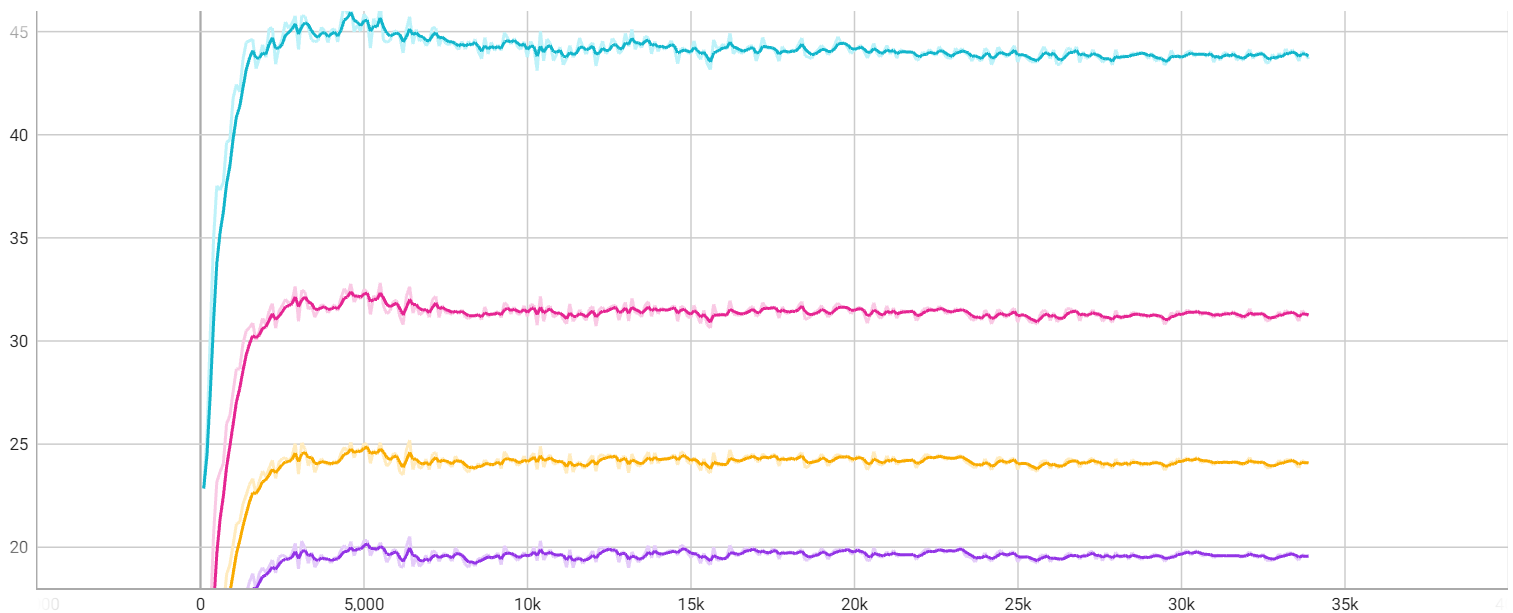
\includegraphics[width=1\textwidth]{../graphics/BlueScoresTraining.png}
    \caption{BLUE scores van het SignFormer model}
    \label{fig:blue-scores}

    \vspace{1cm}

    % Tweede figuur
    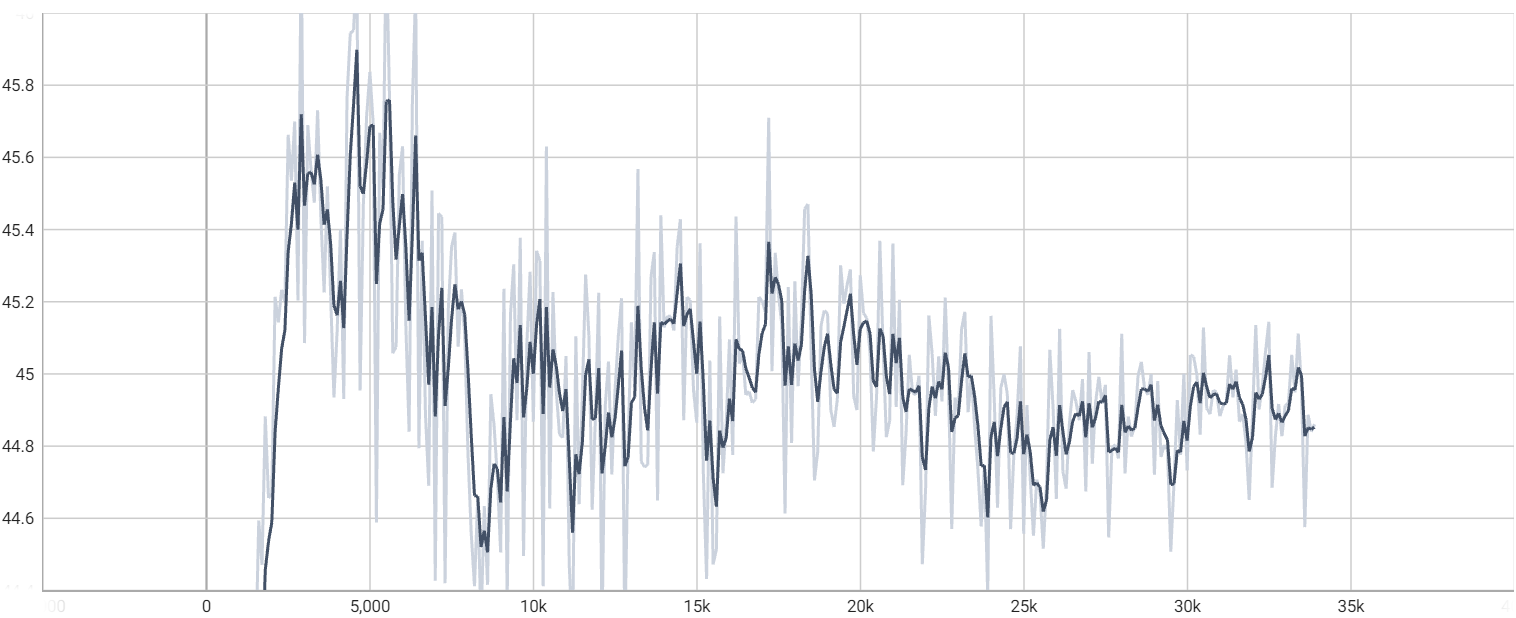
\includegraphics[width=1\textwidth]{../graphics/RougeScore.png}
    \caption{ROUGE scores van het SignFormer model}
    \label{fig:rouge-scores}

    \vspace{1cm} 

    % Derde figuur
    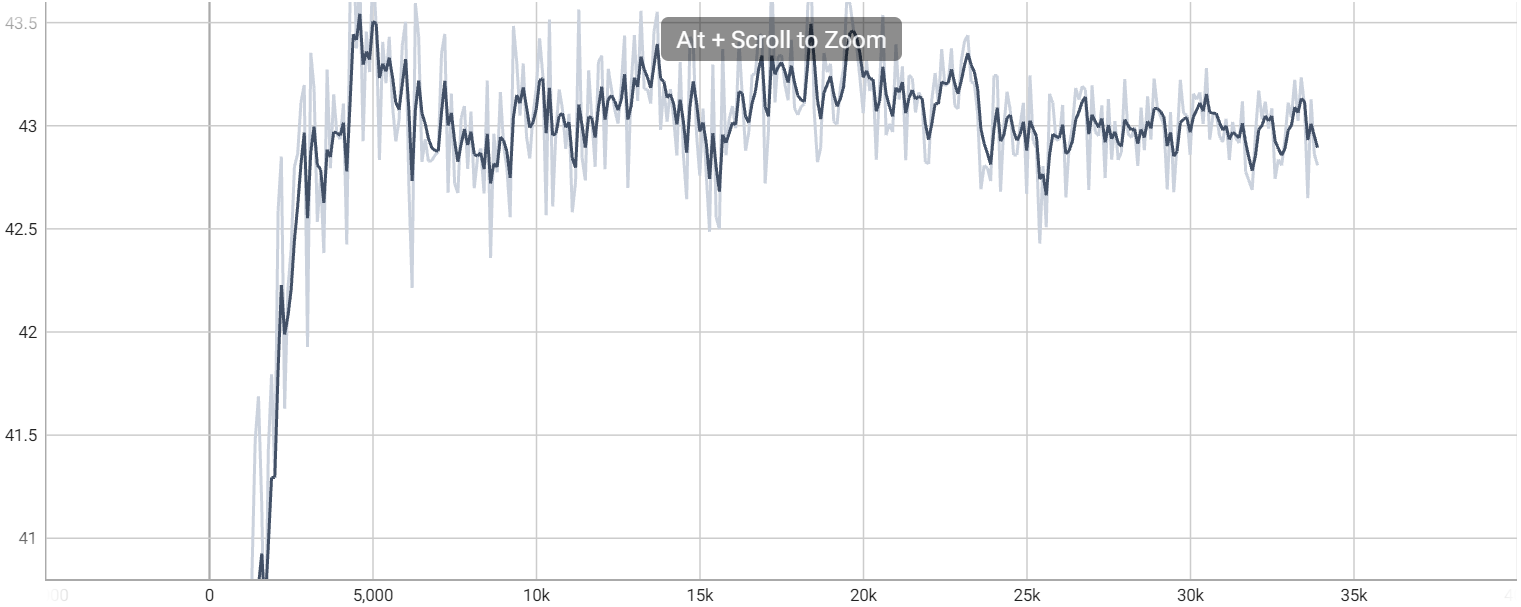
\includegraphics[width=1\textwidth]{../graphics/CHRF.png}
    \caption{CHRF scores van het SignFormer model}
    \label{fig:chrf-scores}
\end{figure}

\chapter{Inferentie op een desktopomgeving}
\label{ch:inferentie}

Voordat een machine learning-model effectief kan worden ingezet op een edge device, is het van essentieel belang om het model eerst uitvoerig te testen op een reguliere desktop- of laptopomgeving.
Deze stap fungeert als een belangrijke tussenfase in het ontwikkelingsproces, omdat edge devices—zoals embedded systemen, mobiele telefoons of microcontrollers—vaak beschikken over aanzienlijk minder rekenkracht, geheugen en energiecapaciteit dan conventionele computers.
Door het model eerst lokaal te testen, kunnen potentiële fouten of inefficiënties vroegtijdig worden opgespoord, zonder de bijkomende beperkingen van een edgeomgeving.
\\
\\
Dergelijke tests maken het mogelijk om inzicht te krijgen in de prestaties, nauwkeurigheid en robuustheid van het model onder realistische omstandigheden.
Bovendien kunnen al in deze fase optimalisaties worden doorgevoerd, zoals modelcompressie, kwantisatie of het herstructureren van de architectuur voor betere compatibiliteit met edgehardware.
Deze voorbereidingen besparen uiteindelijk veel tijd en middelen wanneer het model daadwerkelijk wordt overgezet naar een edge device, en verhogen de kans op een succesvolle, stabiele implementatie.
\\
\\
De manier om inferentie uit te voeren is om een reeks frames te verwerken, waarbij de temporele context van gebarentaal wordt benut. Dit vereist specifieke stappen voor inputvoorbereiding en modeluitvoering.


\section{Inferentie op reeks van frames}
\label{sec:inferentie-reeks-frames}

Door een reeks frames te verwerken in plaats van slechts één frame per keer, kan het Signformer model de temporele context van gebarentaal beter begrijpen.
Dit leidt tot een significante verbetering van de nauwkeurigheid van de vertalingen, omdat het model in staat is om de dynamiek van gebaren over tijd te vangen.
\\
\\
De implementatie van deze aanpak vereist enkele aanpassingen in de manier waarop de input wordt voorbereid, hoe het model wordt aangeroepen, en hoe de output wordt gegenereerd.
Er zijn ook enkele aanpassingen gedaan aan het model zelf waardoor het model veel flexibeler is in het verwerken van de input.
% De inferentie maakt ook gebruik van een sliding window benadering, waarbij een sequentie van frames wordt genomen en de output wordt gegenereerd voor die specifieke sequentie.
% Dit betekent dat het model niet alleen kijkt naar het huidige frame, maar ook een aantal voorgaande frames om de context te begrijpen.
% Hierdoor zal het model een continue stroom van vertalingen genereren, die vervolgens kunnen worden samengevoegd tot een volledige zin of tekst.
\subsection{Aanpassing aan het Model}
\label{sec:aanpassing-model-latex}

Modelaanpassingen omvatten voornamelijk configuratie voor GPU-gebruik en het aanpassen van het interne batching om reeksen frames te verwerken in de encoder en decoder.

\subsection{Sequentie klaarmaken voor het model}
\label{sec:sequentie-klaarmaken-latex}

Een reeks geëxtraheerde frame features moet worden omgezet naar een formaat dat het model begrijpt (een batch PyTorch tensors).
Een functie zoals \texttt{prepare\_sequence\_batch} voert dit uit. 
Kernstappen omvatten:
\begin{itemize}
    \item Stapelen van features en omzetten naar tensors:
    \begin{lstlisting}
        sgn_features = np.stack(sgn_features_list, axis=0) # [seq_len, feature_dim]
        sgn_features = np.expand_dims(sgn_features, axis=0) # [1, seq_len, feature_dim]
        sgn_tensor = torch.from_numpy(sgn_features).float()
    \end{lstlisting}
    \item Verplaatsen naar het juiste device (CPU/GPU).
    \item Aanmaken van een masker om padding te negeren.
    \item Creëren van een minimaal batch-object dat de verwachte model-inputstructuur nabootst voor inferentie.
\end{itemize}

De feature-extractie wordt gedaan met al een reeds bestaand model.
Omdat we niet weten hoe de frames precies zijn gepreprocessed, is het belangrijk om de feature-extractie te doen met een model dat dezelfde preprocessing heeft als het model dat we gaan gebruiken voor inferentie.
Hierbij zijn er meerdere mogelijkheden getest geweest zoals ResNet34, ResNet50, en EfficientNet.
Hierbij is ResNet34 gekozen omdat deze de beste resultaten gaf in de inferentie zowel op snelheid als nauwkeurigheid. 

\subsection{Gedetailleerde Inferentie Uitvoering}
\label{sec:gedetailleerde-inferentie}

De inferentie wordt uitgevoerd in een functie (bv. \texttt{run\_sequence\_inference}) met het geprepareerde batch-object. 
Dit gebeurt in een context die gradiëntbereken\-ing uitschakelt voor efficiëntie:

\begin{lstlisting}
with torch.no_grad():
    decoded_gloss_sequences_ids, stacked_txt_output_ids, stacked_attention_scores = model.run_batch(
        batch=inference_batch,
        recognition_beam_size=args.rec_beam_size, # Voorbeelden van parameters
        translation_beam_size=args.trans_beam_size,
        # ... andere parameters ...
    )
\end{lstlisting}

De \texttt{model.run\_batch} methode voert de forward pass uit (encoder, decoders). 
Parameters zoals 'beam\_size' beïnvloeden de zoekstrategie voor de meest waarschijnlijke output. 
De methode retourneert de identificatiecodes van de voorspelde gloss- en tekstsequenties, en optioneel aandachtsscores.
Deze identificatiecodes worden vervolgens omgezet naar leesbare zinnen met behulp van vocabulaire objecten (bv. \texttt{gls\_vocab}, \texttt{txt\_vocab}):
\begin{lstlisting}
    decoded_gloss_sentences = gls_vocab.arrays_to_sentences(decoded_gloss_sequences_ids)
\end{lstlisting}

\section{Sequentie-gebaseerde Inferentie met Camera Input}
\label{sec:sequentie-inferentie-camera}

Dit gedeelte beschrijft een implementatie waarbij sequentie-inferentie live wordt uitgevoerd met een camerafeed.

\subsection{Argumenten Parsen en Initialisatie}
\label{sec:main-args-init-latex}

Argumenten worden doorgegeven om het gedrag te configureren, zoals het gebruik van de GPU en de sequentielengte:
\begin{lstlisting}
parser = argparse.ArgumentParser(...)
parser.add_argument("--gpu", action="store_true", help="Use GPU")
parser.add_argument("--sequence_length", type=int, default=100, help="Frames per sequence")
# ... andere argumenten ...
args = parser.parse_args()
\end{lstlisting}
De feature extractor en de camera worden geïnitialiseerd:
\begin{lstlisting}
feature_extractor = IntegratedFeatureExtractor(sgn_dim=sgn_dim, use_cuda=use_cuda)
cap = cv2.VideoCapture(args.camera_id)
\end{lstlisting}

\subsection{De Hoofd Inferentie Loop}
\label{sec:main-loop-latex}

Een continue lus leest frames van de camera. Features worden geëxtraheerd en verzameld:
\begin{lstlisting}
collected_features = []
while cap.isOpened():
    ret, frame = cap.read()
    if not ret:
        # Error handling ...
        continue

    features = feature_extractor.extract(frame)
    if features is not None:
        collected_features.append(features)

    # Weergave op frame (status, resultaten) ...
    cv2.imshow('Sign Language Translation', display_frame)

    # Inferentie trigger
    if len(collected_features) >= args.sequence_length:
        print("Running inference...")
        inference_batch = prepare_sequence_batch(collected_features, ...)
        decoded_glosses, translated_text, attention_scores = run_sequence_inference(model, inference_batch, ...)

        # Resultaten verwerken en bufferen...

        collected_features = [] # Wis verzamelde features
\end{lstlisting}
Wanneer voldoende frames zijn verzameld, wordt de sequentie voorbereid en wordt de inferentie uitgevoerd. De resultaten worden getoond op het camerabeeld. De lus stopt bij een toetsaanslag (bv. 'q'):
\begin{lstlisting}
    if cv2.waitKey(1) & 0xFF == ord('q'):
        break
\end{lstlisting}

\subsection{Afsluiting}
\label{sec:main-afsluiting-latex}

Na het stoppen van de lus wordt de camera vrijgegeven en worden vensters gesloten:
\begin{lstlisting}
cap.release()
cv2.destroyAllWindows()
\end{lstlisting}
De code wordt gestart via de standaard \texttt{if \_\_name\_\_ == "\_\_main\_\_":} constructie.

\section{Resultaten}
\label{sec:inferentie-resultaten}
De resultaten van de inferentie zijn veelbelovend.
Het model kan een reeks aan frames verwerken en de bijbehorende gebaren vertalen naar tekst.
De nauwkeurigheid van de vertalingen is laag doordat we niet weten op welke manier de frames zijn gepreprocessed.
De vertaling is dus niet representatief voor de werkelijke vertalingen.
Echter is de snelheid en de tijd die het kost om een sequentie te verwerken wel representatief.
\\
\\
Een groot knelpunt in de inferentie is het inladen van alle verschillende componenten van het model.
Een ander groot knelpunt in de inferentie is de manier van preprocessing van de frames.
Hoe complexer het preprocessing algoritme, hoe meer tijd het kost om de frames te verwerken.
De resultaten zijn gegenereerd met ResNet34 als preprocessing-algoritme en een batch size van 32, gelijk aan die van de training.
\\
\\
Hier ziet U de resultaten van de inferentie \ref{tab:inferentie-resultaten}
\begin{table}
    \begin{tabular}{|l||c|c|c||}
        \hline
        \textbf{Parameter} & \textbf{Min} & \textbf{Gemiddelde} & \textbf{Max} \\
        \hline
        Frame verwerkingstijd (per loop iteratie) & 0.1846s & 0.3360s & 0.8462s \\
        \hline
        Gemiddelde frame rate & 2.98 FPS & 2.98 FPS & 2.98 FPS \\
        \hline
        Feature extractie tijd (per frame) & 0.1745s & 0.3004s & 0.5006s \\
        \hline
        Batch voorbereidingstijd (per sequentie) & 0.0000s & 0.0010s & 0.0021s \\
        \hline
        Model inferentie tijd (per sequentie) & 0.0228s & 0.0587s & 0.1315s \\
        \hline
        Volledige sequentie verwerkingstijd (van begin tot einde) & 6.8808s & 11.0014s & 14.9258s \\
        \hline
    \end{tabular}
    \caption{Resultaten van de inferentie op een reeks van frames.}
    \label{tab:inferentie-resultaten}
    \vspace{1mm}
    {\tiny Resultaten zijn berekent op 69 batches van 32 frames.}
\end{table}
\subsection{Problemen tijdens de Inferentie}
\label{sec:inferentie-problemen}
Tijdens de inferentie zijn er enkele problemen opgetreden die de prestaties en nauwkeurigheid van het model hebben beïnvloed.
Gebarentaal werkt niet opdezelfde manier als gesproken taal.
Bij gebarentaal is het een reeks aan gebaren die samen een zin vormen.
Het is dus niet altijd duidelijk wanneer een reeks aan gebaren eindigt en een nieuwe begint.
Dit kan leiden tot problemen bij het verwerken van de sequenties.
Waarbij er nu bij de inferentie een vaste sequentie lengte wordt gebruikt, zou het beter zijn om een dynamische sequentie lengte te gebruiken.
Dit zou betekenen dat het model zelf kan bepalen wanneer een sequentie eindigt en een nieuwe begint.
Het ander groot probleem dat al eerder is aangekaart is het probleem van de preprocessing van de frames.
Dit is een groot probleem omdat het model niet weet hoe de frames zijn gepreprocessed en dus de vertalingen niet representatief zijn voor de werkelijke vertalingen.
\chapter{Implementatie op Android}
\label{ch:androidSysteem}
\section{Inleiding}
\label{sec:inleiding-android}
In dit hoofdstuk wordt de implementatie van het model op een Android-systeem besproken.
De implementatie is gedaan met behulp van de Android Studio IDE en de Android SDK.
Dit gebeurt in de programeertaal Kotlin.

\section{Voorbereiding voor Inferentie op Android}
\label{sec:voorbereiding-android-inferentie}

Voordat het AI-model voor gebarentaalvertaling effectief kan worden ingezet voor inferentie binnen een Android-applicatie, zijn specifieke voorbereidende stappen vereist die verband houden met het Android-platform en de integratie van machine learning modellen. 
Deze stappen zorgen voor de benodigde toegang tot hardware, de correcte modelformaten en de integratie binnen de applicatiestructuur. 
De belangrijkste voorbereidingen omvatten het volgende:

\subsection{Verkrijgen van de benodigde permissies}
\label{subsec:permissies-aanvragen}

Om video van de camera te kunnen vastleggen voor gebarentaalherkenning, heeft de Android-applicatie expliciete toestemming van de gebruiker nodig. 
Dit vereist configuratie op twee niveaus:
\begin{itemize}
    \item \textbf{Manifest Declaratie:} De benodigde permissie om de camera te gebruiken (\texttt{android.permission.CAMERA}) moet worden gedeclareerd in het \texttt{AndroidManifest.xml} bestand van de applicatie. 
    Dit informeert het systeem dat de applicatie deze functionaliteit vereist.
    \item \textbf{Runtime Permissie Aanvraag:} Voor Android-versies 6.0 (API niveau 23) en hoger, moeten gevaarlijke permissies, waaronder cameratoegang, tijdens runtime expliciet aan de gebruiker worden gevraagd. 
    De applicatie moet logica implementeren om de huidige status van de permissie te controleren, de gebruiker om toestemming te vragen indien nodig, en correct om te gaan met het scenario waarin de gebruiker de permissie weigert.
\end{itemize}
Zonder de juiste cameratoegang kan de applicatie geen videoframes vastleggen en bijgevolg geen inferentie uitvoeren.

\subsection{Model Conversie en Optimalisatie}
\label{subsec:model-conversie}

Het getrainde AI-model, dat mogelijk oorspronkelijk in het framework van PyTorch is ontwikkeld, moet worden omgezet naar een formaat dat efficiënt kan worden gebruikt op mobiele apparaten met beperkte rekenkracht, namelijk PyTorch Mobile.
\begin{itemize}
    \item \textbf{Model Exporteren:} Het getrainde PyTorch-model moet worden geëxporteerd naar een intermediair formaat, vaak via tracing of scripting, dat compatibel is met mobiele conversietools.
    \item \textbf{Conversie naar PyTorch Mobile:} Het geëxporteerde model wordt vervolgens geconverteerd naar het doelformaat (PyTorch Mobile). 
    Dit proces omvat vaak optimalisaties zoals kwantisatie (reduceren van de precisie van de modelgewichten) om de modelgrootte te verkleinen en de inferentiesnelheid te verhogen, wat cruciaal is voor mobiele implementaties.
    \item \textbf{Bestandsvoorbereiding:} Het geconverteerde modelbestand (bijvoorbeeld een `.ptl` of geoptimaliseerd PyTorch Mobile bestand) en de bijbehorende vocabulaire bestanden moeten worden voorbereid en gebundeld met de Android-applicatie, vaak opgeslagen in de 'assets' of 'raw' resources folder van het Android-project.
\end{itemize}
Deze conversie- en optimalisatiestap is essentieel voor het succesvol draaien van het model op de hardware van een Android-apparaat.
\subsubsection{Model Exporteren}
\label{subsubsec:model-exporteren}
Voor de conversie naar PyTorch Mobile moet het model worden geëxporteerd naar een formaat dat geschikt is voor conversie.
Hierbij is het belangrijk dat alle mogelijke uitkomsten van het model worden vastgelegd.
Dit betekent dus als er een None-waarde wordt teruggegeven dit veranderd moet worden naar een lege Tensor.
Dit komt doordat de code die de conversie uitvoert niet kan omgaan met None-waarden.
\\
\\
Als we \textbf{jit.trace} gebruiken om het model te exporteren, moeten we ook een voorbeeldinvoer opgeven die de vorm en het type van de invoer van het model simuleert.
Dit zorgt er echter voor dat het model niet dynamisch is en dat het model niet kan omgaan met verschillende invoerformaten.
Om dit probleem te verhelpen, is het beter om \textbf{torch.jit.script} te gebruiken.
Dit maakt het mogelijk om de modelcode te analyseren en een scriptversie van het model te genereren die kan omgaan met verschillende invoerformaten.
Deze houdt ook rekening met mogelijke if statements in de code.
Dit is belangrijk voor als het model ook andere paden zou moeten volgen, zodat deze ook berekend zijn.
\\
\\
Om ervoor te zorgen dat alle dynamische aspecten van het model correct worden vastgelegd, is het belangrijk om de juiste invoerformaten en -types te gebruiken tijdens het scriptproces.
Dit betekent dus dat bij elke functie waar het type niet goed gespecifi{\"e}erd is en anders kan g{\"e}intreperteerd worden, dit moet worden aangepast.
Dus de volgende stap is de code klaarmaken voor het scriptingprocess. Dit bevat elke variable en elke mogelijke stap die genomen kan worden duidelijk te specifieren.

\subsubsection{Resultaten conversie}
\label{subsubsec:resultaten-conversie}
De conversie van het model naar PyTorch Mobile resulteert in een bestand dat geoptimaliseerd is voor gebruik op mobiele apparaten.
Dit bestand bevat de gewichten en architectuur van het model, maar is geconfigureerd om efficiënt te draaien op de beperkte rekenkracht en geheugen van mobiele apparaten.
De file zal echter groter zijn dan het originele model.
Dit komt doordat de file nu ook de volledige architectuur van het model bevat.
Ook de rekenlogica van het model zitten hierin samen met gespecialiseerde bytecode voor effici{\"e}nte uitvoering.
Het betekent dus waar we in hoofdstuk \ref{sec:training} nog het aantal lagen van het model moesten meegeven en andere parameters, dat dit nu niet meer nodig is.
Het model kan nu ook niet meer verder getraind worden.
Dit zorgt er echter wel voor dat het model bijna direct ingeladen kan worden en dus de tijd die bij de computer infrentie het nodig had niet meer nodig is.
In dit onderzoek is het echter niet gelukt om het model om te zetten naar een formaat dat geschikt is voor edge devices.
Dit komt doordat het model te complex is en veel custom lagen bevat die niet ondersteund worden door PyTorch Mobile.
Wat er dan ook voor zorgt dat het niet makkelijk omzetbaar is naar een ander formaat zoals TensorFlow Lite.
\section{Integratie binnen de Android-applicatie}
\label{subsec:integratie-android}

Het geconverteerde model en de benodigde hulpmiddelen moeten correct worden geïntegreerd binnen de architectuur van de Android-applicatie:
\begin{itemize}
    \item \textbf{Afhankelijkheden Toevoegen:} De benodigde bibliotheken voor het uitvoeren van PyTorch Mobile modellen op Android moeten worden toegevoegd aan de build.gradle bestanden van het project.
    \item \textbf{Model Laden en Initialiseren:} Code moet worden geïmplementeerd binnen de Android-applicatie om het geconverteerde modelbestand van de resources te laden en de inferentie-engine te initialiseren.
    \item \textbf{Camera Integratie:} De camera-API van Android (CameraX) moet worden gebruikt om videoframes vast te leggen. 
    Deze frames moeten vervolgens in het juiste formaat worden aangeleverd aan de invoerlaag van het geladen AI-model.
    \item \textbf{Verwerking van Model Output:} Logica is vereist om de uitvoer van het model te verwerken. 
    Dit omvat het interpreteren van de numerieke output aan de hand van de geladen vocabulaires en het weergeven van de vertaalde tekst op de gebruikersinterface van de applicatie.
\end{itemize}
%%=============================================================================
%% Conclusie
%%=============================================================================

\chapter{Conclusie}%
\label{ch:conclusie}

% TODO: Trek een duidelijke conclusie, in de vorm van een antwoord op de
% onderzoeksvra(a)g(en). Wat was jouw bijdrage aan het onderzoeksdomein en
% hoe biedt dit meerwaarde aan het vakgebied/doelgroep? 
% Reflecteer kritisch over het resultaat. In Engelse teksten wordt deze sectie
% ``Discussion'' genoemd. Had je deze uitkomst verwacht? Zijn er zaken die nog
% niet duidelijk zijn?
% Heeft het onderzoek geleid tot nieuwe vragen die uitnodigen tot verder 
%onderzoek?

\lipsum[76-80]



%---------- Bijlagen -----------------------------------------------------------

\appendix

\chapter{Onderzoeksvoorstel}

Het onderwerp van deze bachelorproef is gebaseerd op een onderzoeksvoorstel dat vooraf werd beoordeeld door de promotor. Dat voorstel is opgenomen in deze bijlage.

%% TODO: 
%\section*{Samenvatting}

% Kopieer en plak hier de samenvatting (abstract) van je onderzoeksvoorstel.

% Verwijzing naar het bestand met de inhoud van het onderzoeksvoorstel
%---------- Inleiding ---------------------------------------------------------

% TODO: Is dit voorstel gebaseerd op een paper van Research Methods die je
% vorig jaar hebt ingediend? Heb je daarbij eventueel samengewerkt met een
% andere student?
% Zo ja, haal dan de tekst hieronder uit commentaar en pas aan.

%\paragraph{Opmerking}

% Dit voorstel is gebaseerd op het onderzoeksvoorstel dat werd geschreven in het
% kader van het vak Research Methods dat ik (vorig/dit) academiejaar heb
% uitgewerkt (met medesturent VOORNAAM NAAM als mede-auteur).
% 
\section{Inleiding}%
\label{sec:inleiding}

\subsection{Vlaams Gebarentaal}
\label{sec:VGT}

In de hedendaagse samenleving is er een groeiende behoefte aan technologieën die de communicatie tussen doven en horenden vergemakkelijken. Een van de meest veelbelovende ontwikkelingen op dit gebied is de real-time vertaling van Vlaamse Gebarentaal (VGT) naar tekst, waarbij gebruik wordt gemaakt van kunstmatige intelligentie (AI) en computer vision. VGT, de taal die door de Vlaamse dovengemeenschap wordt gebruikt, is een volwaardige taal die, net als andere gesproken talen zoals Nederlands en Frans, erkend wordt door de taalkundige gemeenschap. Het is belangrijk op te merken dat VGT, net als gesproken talen, regionale variaties kent, wat de complexiteit van de vertaling vergroot \autocite{vanmeerbergen2000simultane}.

De structuur van VGT is hiërarchisch, wat betekent dat elk gebaar kan variëren in betekenis afhankelijk van specifieke details, zoals handvorm, beweging en gezichtsuitdrukkingen. \autocite{469340}
Deze variabiliteit maakt het noodzakelijk om geavanceerde algoritmen te ontwikkelen die in staat zijn om deze nuances te herkennen en correct om te zetten naar tekst. 
Recent onderzoek heeft aangetoond dat AI-technologieën, zoals deep learning en convolutionele neurale netwerken (CNN), effectief kunnen worden ingezet voor gebarentaalherkenning.\autocite{10.52756/ijerr.2023.v34spl.004}\autocite{10.17485/ijst/v16i45.2583}
Door gebruik te maken van camera's op smartphones en andere apparaten kan een systeem worden ontwikkeld dat in real-time gebaren herkent en omzet in geschreven tekst.
\section{Literatuurstudie}%
\label{sec:literatuurstudie}

% Voor literatuurverwijzingen zijn er twee belangrijke commando's:
% \autocite{KEY} => (Auteur, jaartal) Gebruik dit als de naam van de auteur
%   geen onderdeel is van de zin.
% \textcite{KEY} => Auteur (jaartal)  Gebruik dit als de auteursnaam wel een
%   functie heeft in de zin (bv. ``Uit onderzoek door Doll & Hill (1954) bleek
%   ...'')

%---------- Methodologie ------------------------------------------------------
\section{Methodologie}%
\label{sec:methodologie}


%---------- Verwachte resultaten ----------------------------------------------
\section{Verwacht resultaat, conclusie}%
\label{sec:verwachte_resultaten}


%%---------- Andere bijlagen --------------------------------------------------
% TODO: Voeg hier eventuele andere bijlagen toe. Bv. als je deze BP voor de
% tweede keer indient, een overzicht van de verbeteringen t.o.v. het origineel.
%\input{...}

%%---------- Backmatter, referentielijst ---------------------------------------

\backmatter{}

\setlength\bibitemsep{2pt} %% Add Some space between the bibliograpy entries
\printbibliography[heading=bibintoc]

\end{document}
